\documentclass[]{algotel}
\usepackage[utf8]{inputenc}
\usepackage[english]{babel}

\usepackage{xspace}
\usepackage{graphicx,graphics} 
\usepackage{mathtools, bm}
\usepackage{caption}
\usepackage{amssymb, bm}
\usepackage{complexity}
\usepackage{amsthm}
%\usepackage{authblk}
\usepackage{color}
\usepackage{amsmath}
\usepackage[colorlinks=true,breaklinks=true,linkcolor=blue]{hyperref}

\captionsetup{justification=centering,margin=0.5cm}

\newcommand\pall{\textsc{pall}\xspace}


\newcommand{\todo}[1]{{\color{red} TODO: {#1}}}	
\newtheorem{prop}{Proposition}
\renewcommand{\thefootnote}{\*}


\graphicspath{{img/}}

%opening
\title{Contention management for Cloud RAN over an optical ring}

%\author[1]{Dominique Barth}
%\author[2]{Dominique Chiaroni ?}
%\author[1]{Ma\"el Guiraud}
%\author[1]{Yann Strozecki}
%\affil[1]{David Laboratory, UVSQ}
%\affil[2]{Nokia Bell Labs France}




\author{Dominique Barth\addressmark{1}
  \and Ma\"el Guiraud\addressmark{1}
   \and Yann Strozecki\addressmark{1}
  }

\address{\addressmark{1}David Laboratory, UVSQ}
% \\
%   \addressmark{2}Nokia Bell Labs France}
\keywords{Optical ring, Latency, C-RAN, SDN}

\begin{document}

\maketitle


\begin{abstract}

% Nowadays challenge for network providers is to design some network which satisfies in the same time a good Quality of Services and a cheap hardware development.
N-GREEN project has for goal to design a low cost optical ring technology with good performances (throughput, latency$\dots$) without using expensive end to end connections. We study the compatibility of such a technology with the development of the Cloud RAN, a latency critical application which is a major aspect of 5G deployment. We show that deterministically managing Cloud RAN traffic minimizes its latency without impacting the latency of others traffics. 
\end{abstract}


\section{Introduction}
 \footnote{ This work was developed around the ANR N-GREEN project. The authors thank the Nokia Bell Labs team for their collaboration.} 

Network providers have to design inexpensive networks while the amount of data and online applications significantly increases. Much of these applications have QoS criteria, like a minimal throughput or a maximal latency. The N-GREEN project aims to design a high performing optical ring while ensuring a minimal cost for providers. The current solutions with good QoS~\cite{pizzinat2015things}, establishes end to end connection (E2E) between the nodes, which is extremely expensive. The N-GREEN optical ring is designed to ensure good performances and the hardware it requires scales linearly with the number of nodes while E2E scales quadratically making it impractical for more than a few nodes.

In this article, we study a Cloud RAN (C-RAN) application in the N-GREEN optical ring described in~\cite{ngreenarchitecture}. C-RAN is one of the major area of development for 5G, that consists in centralizing the computation units or {\bf BaseBand Units} (BBU) of the {\bf Remote Radio Heads} (RRH) in one datacenter. The latency of the messages between the BBU and the RRH is critical~\cite{bouguen2012lte,3gpp5g}. In this article we propose a SDN approach to deterministically manage the periodic C-RAN traffic by chosing emmission timing and reserving containers on the ring. In a previous work~\cite{dominique2018deterministic}, the authors have studied this problem for a star shaped network. Here the load due to the CRAN traffic is small which makes the problem easier. However, we add several new difficulties: the messages from RRHs are fragmented, there are other traffics which must not be impacted and the broadcast and select policy of the ring makes reservation of a specific time for emission somewhat wasteful. 

In Sec.~\ref{sec:model}, we model the optical ring and the traffic flow. In Sec.~\ref{sec:oportmethods}, we study the latency when using stochastic multiplexing to manage packets insertions on the ring, with or without priority for C-RAN packets. In Sec.~\ref{sec:deterministicalgorithms}, we propose deterministic ways to manage C-RAN packets without buffers and thus with a minimal latency compared to stochastic multiplexing. The best method to do so also improves the latency of best effort packets.

\section{Model of C-RAN traffic over an optical ring}
\label{sec:model}
% 
%   \subsection{Network modeling}
% 
% The model exposed here has already been studied for another particular topology of network and with different problematics from the ones of this paper. One can find in \cite{latency2017} the complexity results on the problem proposed, and some algorithmic solutions to solve it in star networks.
          
  \paragraph{N-GREEN Optical ring}
   
  The unidirectional optical ring is represented by an oriented cycle. The vertices of the cycle represents the nodes of the ring, where traffic arrives. The edges $(u,v)$ of the cycle have an integer weight $\omega(u,v)$ which represents the time to transmit a unit of information from $u$ to $v$. By extension, if $u$ and $v$ are not adjacent, we denote by $\omega(u,v)$ the size of the directed path from $u$ to $v$.  We denote by $RS$ (ringsize) the length of the cycle, that is $\omega(u,u)$.  Each arc $(u,v)$ can be seen as a sequence of $\omega(u,v)$ {\bf containers}, of capacity $C$, expressed in Bytes.  The containers are filled by the nodes. The node $u$ can put some data in the first container of the arc $(u,v)$ \emph{only if it is free}. 
  The dynamic of the network is simple: at each unit of time, data contained in a container go to the next.
   The ring follows a {\bf broadcast and select with emission release policy}. When a container is filled by some node $u$,
   it is freed when it comes back at $u$ after a whole round trip.
%    \todo{on ne parle pas assez de la periode je trouve}
   
   \paragraph{C-RAN traffic}
   
   The RRH are the source of the \emph{deterministic and periodic} C-RAN traffic.
   There are $n$ RRHs attached to the ring, the RRH $i$ being attached to the vertex $u_i$ (several antennas can be attached to the same vertex). An RRH is linked to a node of the ring through an electronic interface of bit rate $R$ Bps.
   The ring has a larger rate of $F\times R$ Bps. The integer $F$ is called the {\bf acceleration factor} between the electronic and the optical domains. A node aggregates the data received on the electronic interface during $F$ unit of times to create a packet of size $C$ which completely fills one container of the ring. Each period $P$, an RRH emits a C-RAN traffic 
   during a time $ET$ (emission time), which consists in a packet of size $C$ each $F$ unit of times.
   
   The data of the RRH $i$ arrives at node $u_i$ at a time $m_i$ called its {\bf offset}. The offsets can be determined 
   by the designer of the system and can be different for each RRH but must remain the same over all periods. We assume that all 
   BBUs are contained in the same data-center attached to the node $v$. The data from $u_i$ is routed to its BBU at node $v$ through the ring and arrives at time $m_i + \omega(u_i,v)$ if it has been inserted in the ring upon arrival. Then after some computation time (which is supposed to be zero to simplify the presentation), an answer is sent back from the BBU to the RRH. The same quantity of data is emitted by each BBU or RRH during any period.
   The {\bf latency} of a message is the time it waits in a node before being put in a free container on the ring.
   The aim of our study is to minimize the latency of the C-RAN traffic, both from the RRHs and the BBUs. 
   In Sec.\ref{sec:deterministicalgorithms} we propose a deterministic mechanism with zero latency. 
   The only downside is that other data use the optical ring and their latency may be increased. We shortly describe the
   nature of this additional traffic in the next subsection.
   
    
\begin{figure}[h!]
\begin{center}   

      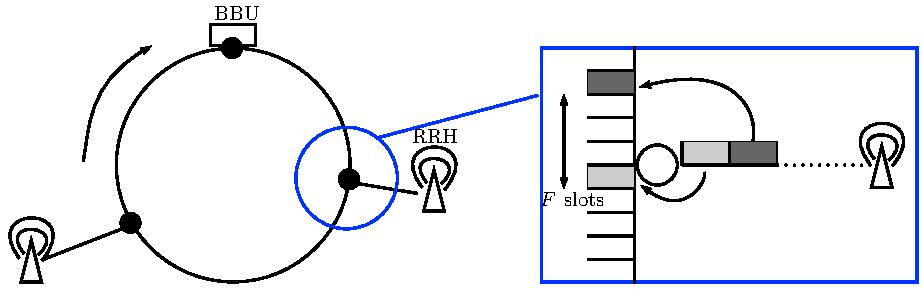
\includegraphics[scale=0.8]{interface.pdf}
     \caption{Opto-electronic interface.}
     
\end{center}
  \end{figure}
    
%       An node deals with two kinds of traffics. Some C-RAN and some Best Effort. We assume that each traffic has its corresponding electronic interface. Also, a C-RAN message is of size $Z$ and completely fills a container let us call {\bf C-RAN PDU} such a message. In the same time, the Best Effort messages are buffered in a first {\em gathering buffer} before being gathered together into a {\bf BE PDU}. Once the PDUs are created, there join the {\em contention buffer} before being sent in the ring.  
%       \begin{figure}[h!]
% \begin{center}   
%   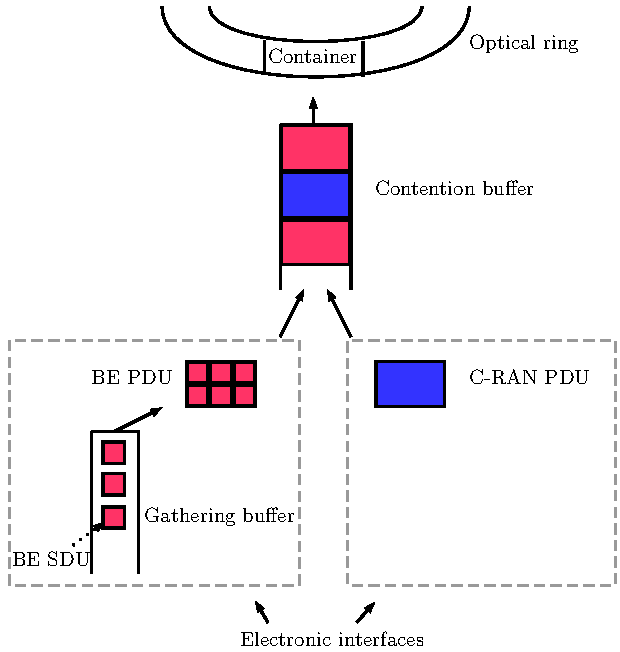
\includegraphics[scale=0.7]{buffers.pdf}
%      \caption{An N-GREEN station.}
%      
% \end{center}
%   \end{figure}
%  
   
%    
%   The C-RAN PDUs coming from an antenna are sent according to a 
%   
%   follows 
%   This study focuses on the performances of the C-RAN PDUs, thus the route we consider are the routes between the BBUs and the RRHs .We assume that there is a bijection between the RRHs and the BBUs.
%  We call forward routes the routes going from the RRHs to the BBUs and Backward routes the routes going from the BBUs to the RRHs. The addition of the weight of the two routes of a couple BBU-RRH is then equal to $RS$, the size of the ring, measured in slots. We denote by $n$ the number of couples BBU-RRH.
%  We only consider one data center into the ring. This mean that all the forward routes have the same destination nodes, and all the backward routes have the same source node.

% 
% 
% \subsection{Into the node : Two kind of traffics}



\paragraph{Best effort traffic}

The optical ring supports other traffics, corresponding to the internet flow. We call this traffic \textbf{Best Effort} (BE), since it is less critical and one can increase the latency of BE messages to improve the latency of C-RAN messages. 
A contention buffer is filled by a batch arrival process of BE data. Then according to some parameters (fill rate and maximum wait time) a container is sent on the ring from the contention buffer. The arrival of BE messages is modeled by a temporal law that gives the distribution of times between two arrivals of a container of BE messages in a node. This distribution is obtained by choosing optimal parameters for the contention buffer~\cite{}. 

% 
% 
%   \subsection{Parameters of the study}
%   \label{sec:parameters} The experiment of this subsections are made following the same parameters, until sec~\ref{sec:optialgo}. We set $K = 10$ chanels, some electronic interface of rate $D=10$Gbps and $Z = 12500$B so, $Z/KD = 1\mu$s. The optical ring has a rate $KD=100$Gbps, while a slots has a duration of $1\mu$s. The length of the ring is to $20$km in our simulations, this means that the ring has a length of $RS = 100$ slots. We consider some BE SDUs of $125$B, and we parametrized BE PDU generator of sec~\ref{jmf} such that each node load the network with an average of $3,5\%$ of BE traffic. We set $ET = 500$ slots, that correspond to a C-RAN traffic of $5$Gbps. The period  $P$ is to $1$ms, that is $1000$ slots. We set the number of RRH to $n=5$. We take $5$ nodes and one of them is the datacenter. The antennas are apportioned between the others node. With those parameters, the network is theoretically loaded to $67.5\%$. 
%   

  
   \section{Performance evaluation of the N-GREEN optical ring}
   \label{sec:oportmethods}
   
   
   
  One first study the latency of the C-RAN and BE traffics when the ring follows an opportunistic insertion policy: when a node wants to send some data, it uses the first free container available on the ring. 
  If a node cannot send a container, because there is no free slot or because several containers must be sent at the same time, the remaining containers are stored in an insertion buffer. Two different methods to manage this insertion buffer are experimentally compared. The FIFO rule is compared to another method that uses two insertion buffers: one for the containers with BE data, and another for the containers with C-RAN data. If there is a free container on the ring, the node empties the C-RAN insertion buffer first.  Fig.~\ref{fig:resultopport} gives the cumulative distribution of both C-RAN and BE traffics latencies for the FIFO rule and the "C-RAN first" rule. On this experiment, the offsets of the RRH are not fixed but randomly drawn in the period. The experimental parameters are given by Fig.~\ref{fig:params} and chosen following~\cite{ngreenarchitecture}. The results are computed over $100$ instances of optical rings that are simulated during $10,000,000$ unit of time.
  
    \begin{minipage}[b]{0.50\linewidth}


        \begin{center}
      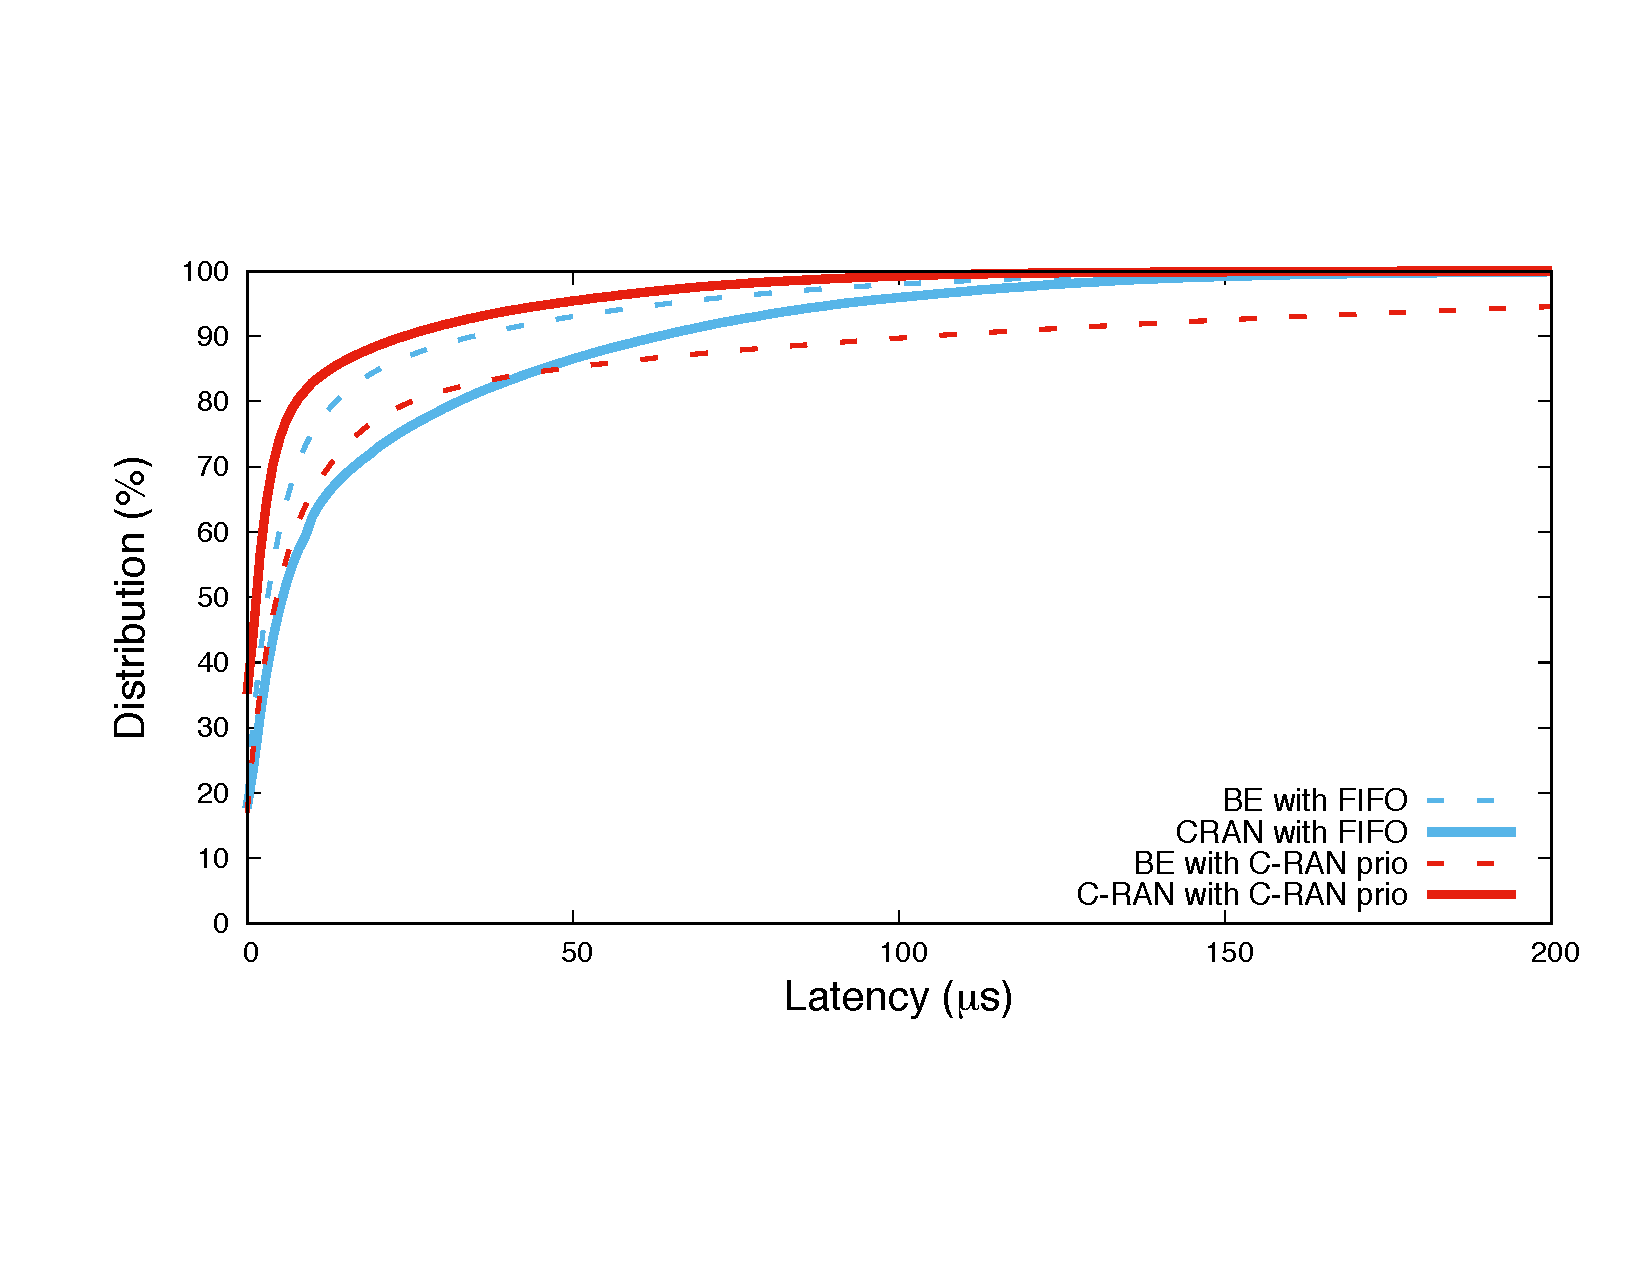
\includegraphics[scale=0.3]{opport.pdf}

      \captionof{figure}{Performances of FIFO and C-RAN first.}    \label{fig:resultopport}
      \end{center} 
  \end{minipage}
\hfill
  \begin{minipage}[b]{0.40\linewidth}
  \vspace{-2cm}
  \scalebox{0.7}
  {
  \centering
  \begin{tabular}{|c|c|}
  \hline
 Acceleration factor $F$ & $10$  \tabularnewline
  \hline
  Bit rate of an electronic interface $R$ & $10$ Gbps \tabularnewline
  \hline
  Container size  $C$ & $12,500$ B  \tabularnewline
  \hline
  Slot duration $C/F\times R$ & $1\mu$ s \tabularnewline
  \hline
  Optical ring bit rate $F\times R$ & $100$ Gbps \tabularnewline
  \hline
  Length of the ring $RS$ & $100$ \tabularnewline
  \hline
  Emission time $ET$ & $500$ \tabularnewline
  \hline
   Period $P$ & $1,000$ \tabularnewline
  \hline
  Number of RRH & $5$  \tabularnewline
  \hline
  Number of nodes $n$ & $5$  \tabularnewline
  \hline
  \end{tabular}
  }
  \vspace{0.75cm}
  \captionof{figure}{Parameters experiments from the N-GREEN architecture}\label{fig:params}

  \end{minipage} 
  
Unsurprisingly, the latency of the C-RAN traffic is better when we prioritize the C-RAN messages, while the BE traffic is penalized. Nevertheless, there is still $10\%$ of the C-RAN traffic with a latency higher than $50 \mu$s, a problem we address in the next section.


%    
%    
%    \subsection{Full opportunistic method}
%    \label{sec:fullopport}
%    We first want to look at a simple configuration in which we do not manage the PUDs (BE or C-RAN) arriving into a node. At their arrival, the BE and C-RAN PDUS are buffered in the contention buffer, and this buffer is emptied following the FIFO rule.
%
%The following experiment shows us the performance this {\bf full opportunistic method} with some parameters issued from N-GREEN. 
%On fig~\ref{fig:oport}, one can see the cumulative distribution of the latency of the C-RAN and BE PDUs.  The measures are taken after $3,000$ slots of simulation, to let the ring initialize it's behavior. The parameters of the simulations are stated in sec~\ref{sec:parameters}.
%
%
%    \begin{figure}[h!]
%    \label{fig:oport}
%        \begin{center}
%      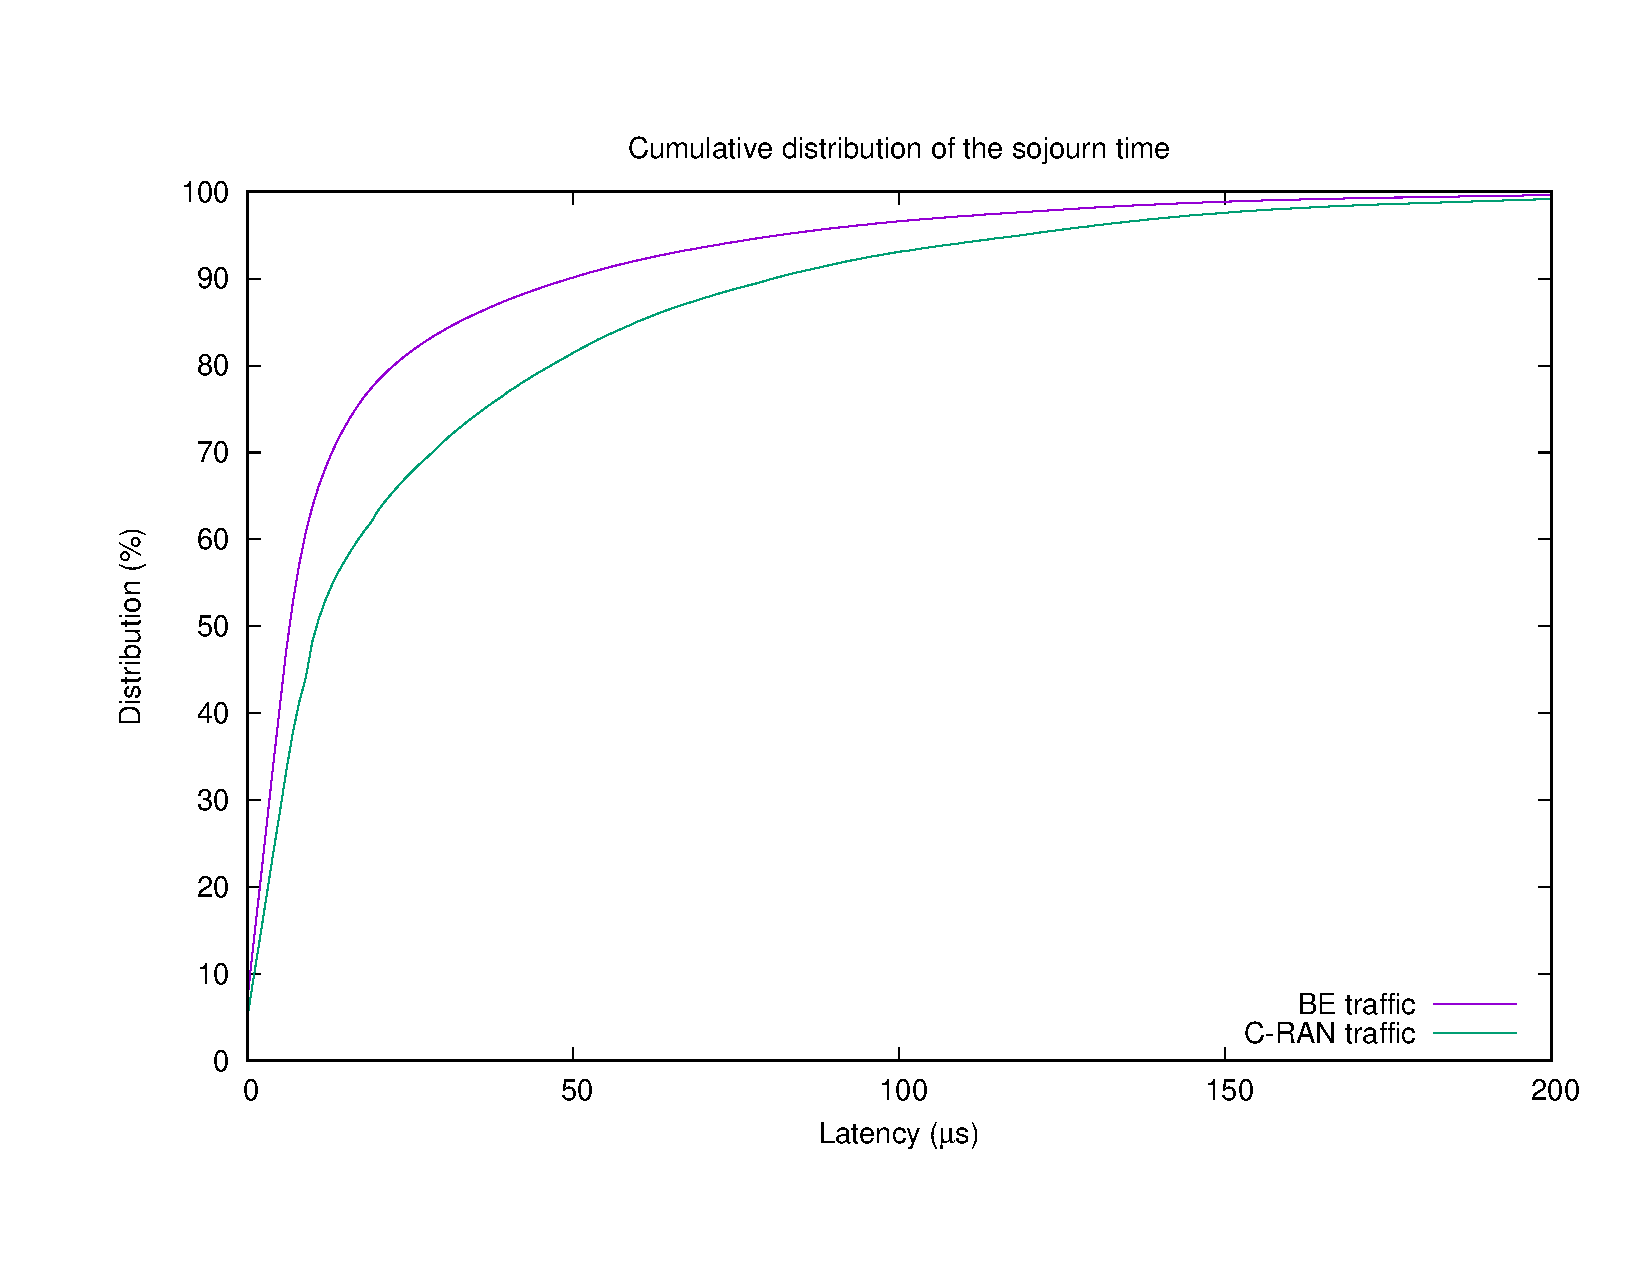
\includegraphics[scale=0.4]{oport}
%
%      \caption{Full opportunistic method performances.}
%      \end{center}
%  \end{figure}
%  
%  As we can see on fig~\ref{fig:oport}, the latency for the different kind of PDU is notably similar because we do not manage anything. Furthermore, we can remark that about $10\%$ of the C-RAN messages wait over $100\mu$s, that is already critical for C-RAN \todo{ref}.
%
%\subsection{C-RAN priority method}
%\label{sec:cranprio}
%  In order to improve the C-RAN PDUs latency, we imagined the following solution, called {\bf C-RAN priority method}. Each nodes have two contention buffers. One for the BE PDUs, and one fore the C-RAN PDUs. When a node is able to send a PDU on the ring, i.e. its available container is free, the container is filled with the C-RAN PDUs first. 
%  
%    \begin{figure}[h]
%\begin{center}   
%      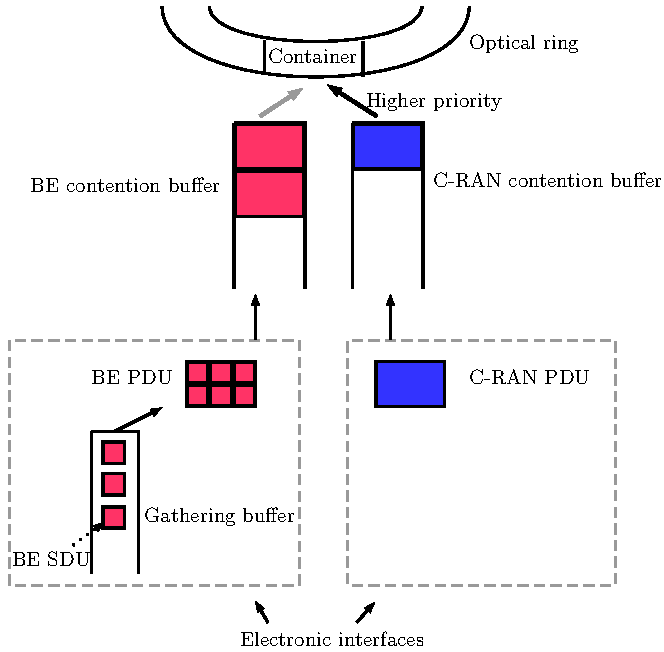
\includegraphics[scale=0.7]{cranprio.pdf}
%     \caption{C-RAN priority method.}
%\end{center}
%  \end{figure}
%  
%  With this method, one can imagine improve the latency of the C-RAN PDUs. Fig~\ref{fig:prior} shows us the performance of the C-RAN priority algorithm for different kinds of traffics. The parameters of the simulations still the same, stated in sec~\ref{sec:parameters}.
%      \begin{figure}[h]
%      \label{fig:prior}
%\begin{center}   
%
%      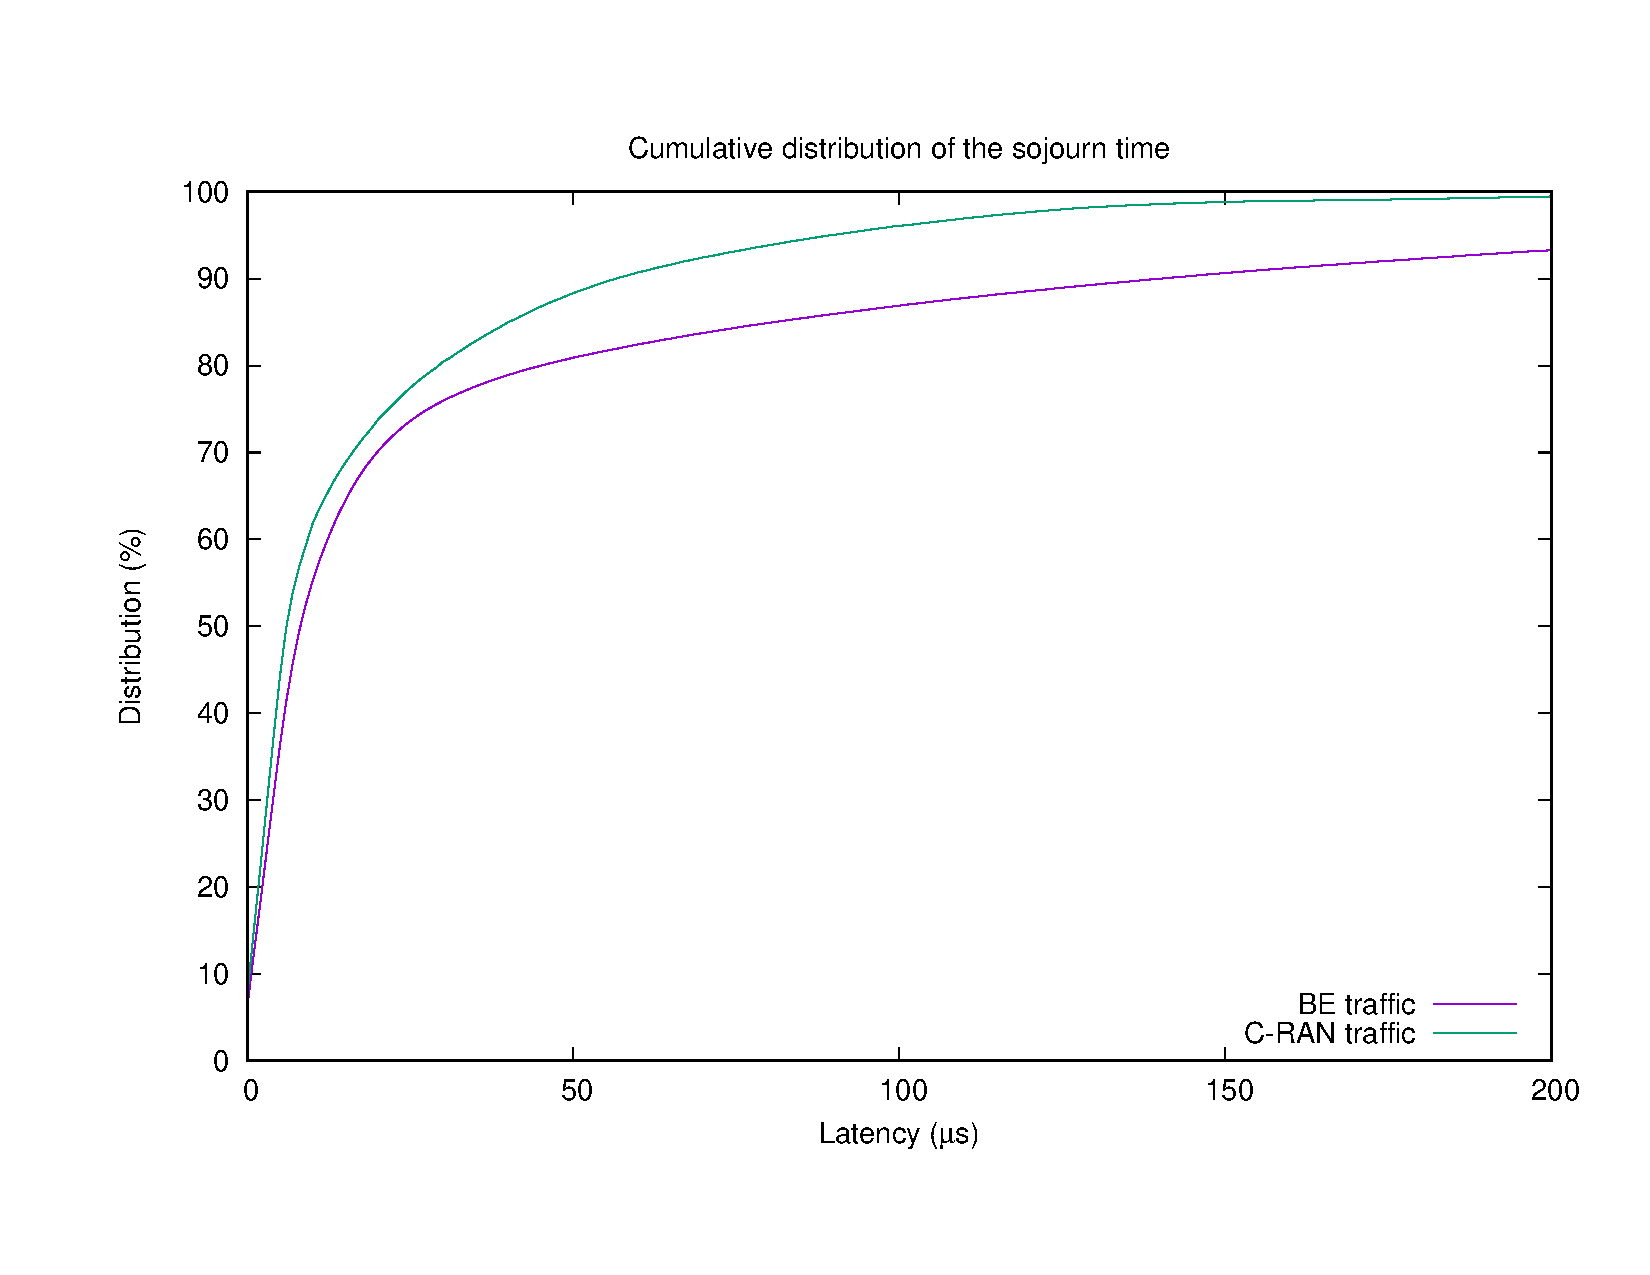
\includegraphics[scale=0.4]{prior.pdf}
%
%     \caption{C-RAN priority method performances.}
%\end{center}
%  \end{figure}
%  
%  As expected, the latency of the C-RAN PDUs is decreased compared to the full opportunistic method. Nevertheless, there is still $10\%$ of the C-RAN PDUs that have more than $50 \mu$s of latency, and the best effort PDUs are penalized, indeed, close to $10\%$ of the BE PDUs awaits more than $150\mu$s before being sent in the ring, versus close to $0\%$ with the previous method..
%  Thus, we propose a deterministic approach in which we set the offsets of the RRH and we reserve the containers needed for the C-RAN PDUs.
%   \todo{il manque une partie sur le travail de karim, }


  \section{Deterministic approach for $0$ latency on C-RAN}
\label{sec:deterministicalgorithms}

Some studies have already been made in order to set the offsets of C-RAN traffic for a different topology~\cite{dominique2018deterministic}. It appears that this problem is not hard in the N-GREEN optical ring. Therefore, one must try to set the offsets for C-RAN traffic such that the BE-traffic latency be not impacted too much.

In order to ensure $0$ latency for C-RAN, the container needed to send a C-RAN message from the RRH $i$ must be free at time $m_i$. Consequently the node reserve the written access this container at time $m_i - RS$. Thus, during the last round trip of the container before $m_i$, the others nodes can only free the reserved containers.

Since the computation time of the BBU is supposed to be zero (or a multiple of the period), setting the offsets $m_i$ for all RRH $i$ also sets the time $m_i + \omega(u,v)$, called {\bf BBU offset}. Because all the BBU are located in the same datacenter, setting the BBU-offsets without coliisions directly avoid the collision between the C-RAN. A {\bf macro slot} is a sequence of $F$ slots. A RRH can emit at most once every macro slot but requires two free containers (one for the uplink message, and one for the downlink one) to ensure zero latency. A {\bf pair} is a sequence of two consecutive slots in the macro slot, the messages of two RRH assigned to different pair can not collide.

\begin{prop}
 If several RRH shares a pair, it is possible to set the BBU-offsets such that there is no collisions between the messages if $P \ge n\times ET + RS$.
 \end{prop}
 \begin{proof}
One show that proposition by induction.
 In this proof, the model is simplified in order to study the behavior of one pair, thus, both of the RRH emit some containers every slots, during $ET$ slots in the period $P$.
 {\bf Base case:} 
 Consider $P =  2.ET+RS$ and two RRH each connected to the nodes $A$ and $B$.
 We assume that $A$ starts to emit a time $1$ during $ET$ slots. The containers of $A$ arrive in $B$ during the interval $[\omega(A,B);\omega(A,B)+ET[$. Then, $B$ can immediately emits its containers at time $\omega(A,B)+ET$. Those containers from $B$ arrives at $A$ at during  $ [\omega(A,B)+ET + \omega(B,A) ;\omega(A,B)+ET + \omega(B,A) + ET ] = [ET+RS;2.ET+RS] = [ET + RS; P]$. Then, $A$ can emit in the next period, without collisions.
Thus, for $n = 2$, it is possible to assign two RRH on the same pair if $P = 2\times ET + RS$.
 
 {\bf Induction step:}  A ring can support $n$ RRH with a period of size $P= n\times ET + RS$. One must show that if there is one more RRH on the ring, the period must be at least $P = (n+1)\times ET + RS$. 
 
Take a sequence of container of size $P$ on a ring with $n$ RRH. One can observe that this sequence is the same at every nodes, shifted of the length of the routes between the nodes. For instance, with two nodes $A$ and $B$, the sequence in $A$ is the same that the sequence in $B$ shifted by $\omega(A,B)$.
In addition if the sequence is increased by $ET$ free containers, the periodic emissions of all others nodes are not impacted, there is just a new interval in the sequence to carry the traffic of a new RRH. Thus a period $P = (n+1)\times ET + RS$ is enough to carry the traffic of $n+1$ RRH.
 \end{proof}

For the purpose of decreasing the BE traffic latency, it is interesting to regularly ensure some free pairs for the BE messages. To this end, the pairs must be filled with as much RRH as possible. Then, the free pairs are uniformly apportioned into the macro slot. Nevertheless, this is not always enough to ensure a good BE traffic latency. Indeed, with the previous parameters, with $ET = \frac{P}{2}$, $F = 10$ and $n = 5$, a pair is given to each antenna, and if all the RRH starts to emit in the same macro slots, a long sequence of reserved container will highly impact the latency of the BE traffic. The solution to this issue is to uniformly distribute the BBU-offset of the first RRH of a pair on the period. In this situation, the number of free pairs in a macro slot is balanced on the period, that allows a more regular BE traffic. Fig.~\ref{fig:optimres} is a compariason between the cumulative distribution of the BE traffic latency with the FIFO rule or with the reservation algorithm proposed here. Since the previous parameters were too restrictive to put several RRH on the same pair, the parameters $ET$, and $n$ have been changed to respectively $200$ and $12$, to keep the same expected load.
   \begin{figure}[h]
\centering
      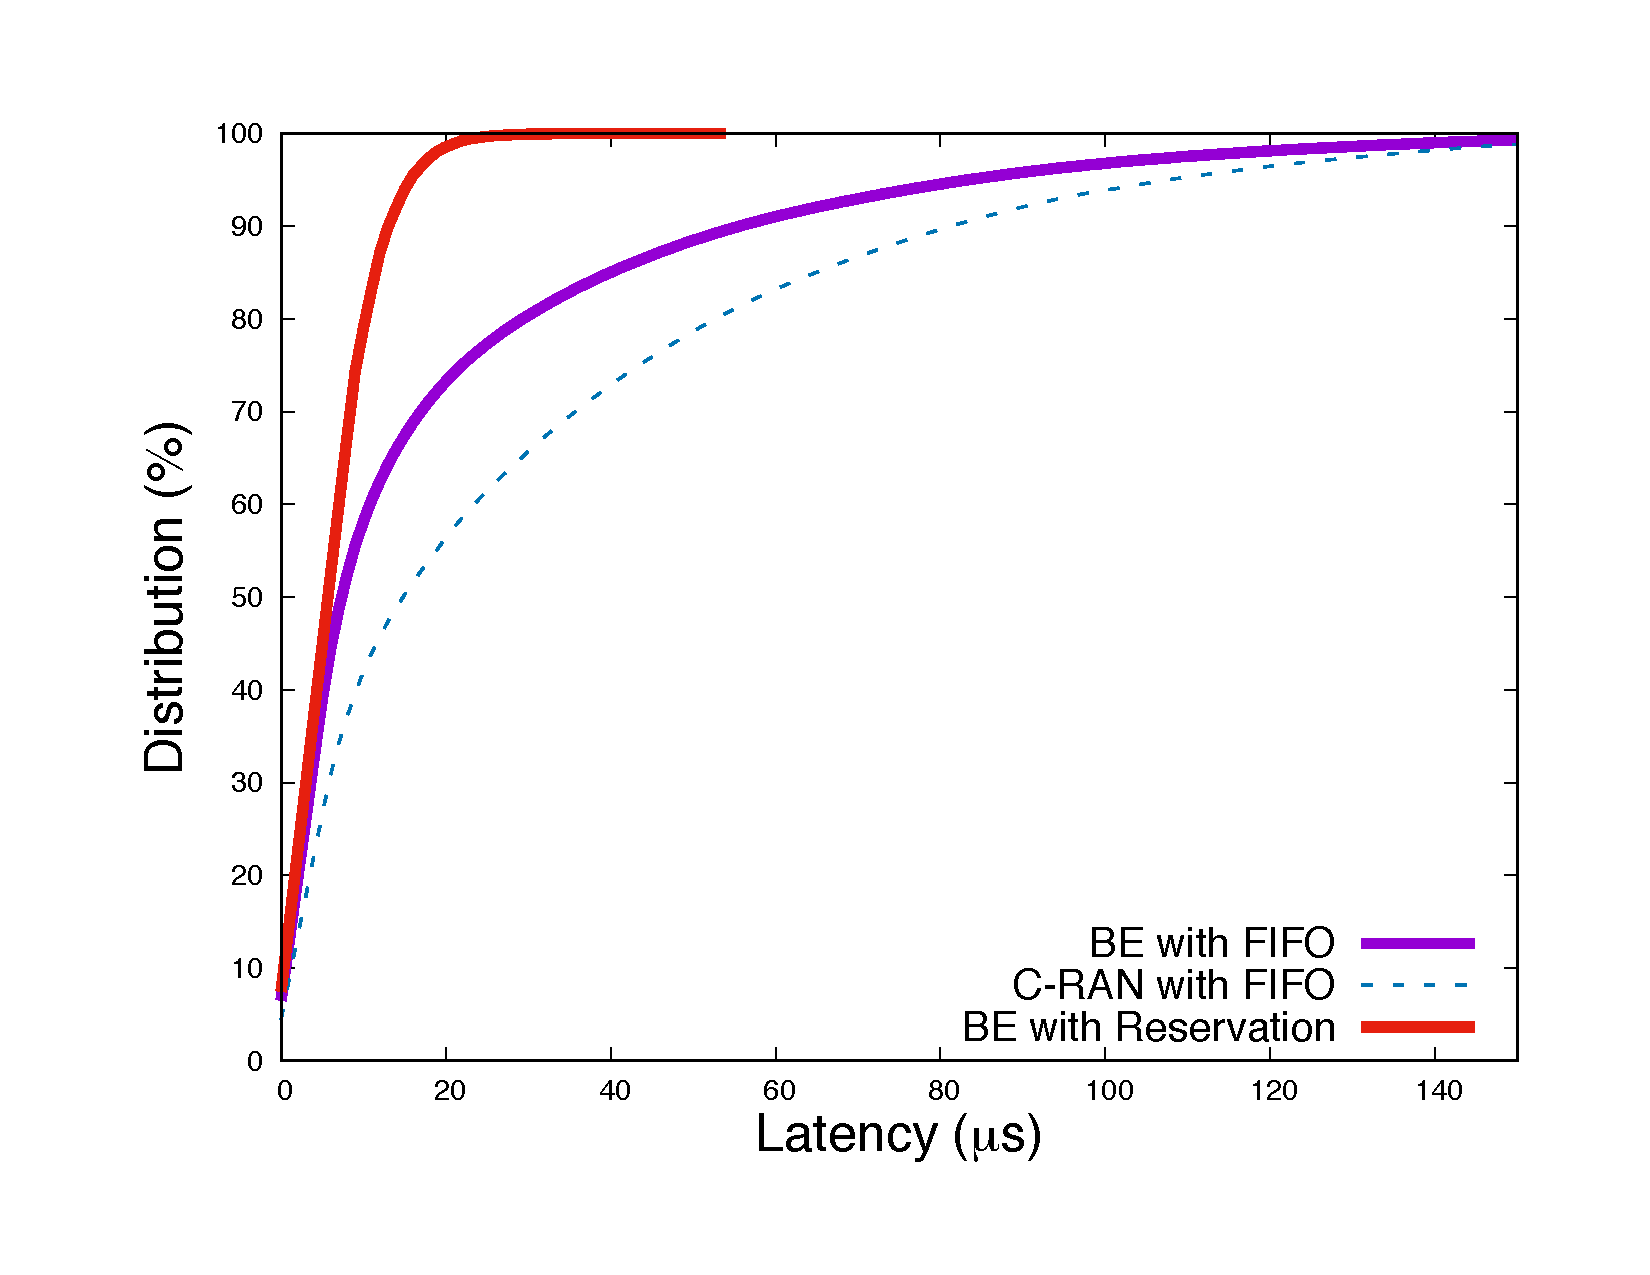
\includegraphics[scale=0.3]{optim.pdf}
     \caption{Impact of the reservation of the traffics.}   \label{fig:optimres}
  \end{figure}
  The performances are excellent, since the C-RAN traffic have $0$ latency and the BE traffic have a better latency with reservation than with the FIFO rule. Indeed, our algorithm balanced the load of the C-RAN traffic over the period , that helps the BE traffic to not aggregate and create additional latency.
  

%% In this section We present three algorithms that allows the C-RAN PDUs to have $0$ latency in the insertion buffers by establishing a static reservation of the slots in the period.
%% Those algorithm are {\bf Centralized} and requires a global supervisor of the network to be implemented .\todo{phrase + ref sdn?}
%% 
%%\paragraph{Slot reservation} To decrease the C-RAN messages latency, one plan to reserve the container for the nodes. Indeed, if a node $i$ needs to send a PDU at time $t$, a container needs to be reserved since the previous lap of the container, i.e. at time $t - RS$ by $i$. In this situation, if the container is already taken by a PDU which has been sent by a node $j$, $j$ will remove the PDU of the container during the next lap of the ring, and no other nodes are able to write in this container before it comes back to the node $i$ a date $t$. By choosing the offsets of the route and reserving the corresponding containers, we allow the C-RAN PDUs to have $0$ latency in the nodes. Though, it impacts the best effort PDUs, by avoiding them to use free reserved containers. It is equivalent to increase the load of the network, without increasing the number of PDUs carried by the network. 
%%
%%\paragraph{RRHs synchronisations}
%%This slot reservation implies that the RRHs are synchronized with the ring. The following proposed algorithms set a sequence of reserved slots for each RRH in each period. A technical application implies to simultaneously ensure the reservation of the slot to the given dates, and the synchronization of the RRH with those reserved slot. One must ensure that the C-RAN PDU arrives in the contention buffer of the node just before the reserved container.
%%
  
%Unlike the previous methods with opportunistic insertion policy, we now want to choose a the offsets for the routes. Since all the forward routes have the same last vertex $v$ (the datacenter), which is also the first vertex of all the backward routes, we choose to manage the collision in this vertex only. The purpose is then to determine the time BBU offset of the routes. Once the BBU-offsets are set, for all routes $i$, it is easy to compute $m_{r_i} = t(v,r_i) - \omega(u,v)$.
%
%
%\subsection{N-GREEN parameters adapted algorithms}
%An RRH can not emit a message more often than once slot every $K$ slots. Remember that {\bf macro slot} is a duration of $K$ slots, during which each RRH can emit at most once. Thus, we consider the simple case in which there is less C-RAN traffic than slots in a macro slot. Indeed, in that case, we only manage the collision in one macro slot, i.e. we assign a C-RAN traffic to each slot of the macro-slot. Since a BBU always instantly emits an answer to it's RRH, for each RRH, a group of two following containers (called {\bf bunch}) can be reserved. Thus, we first study the case $K \ge 2\times n$. As a reminder, $n$ is the number of couple BBU-RRH. 
%
% 
% Because there is at most as much couples BBU-RRH as bunches, we want to assign one RRH to one bunch.
%We propose the following {\bf naive reservation algorithm}. For each RRH $i, i\in \{0,...,n-1\} $, set $t(v,r_i)= 2\times i$ with $v$ the vertex of the BBUs. The model automatically fixes the offset of the backward route $\rho(r_i)$ to $m_{\rho(r_i)}= 2\times i +1$. This is the reason why we do not care about the backward routes anymore, and we only deal with the BBU-offsets of the forward routes..
%   \begin{figure}[h]
%\centering
%      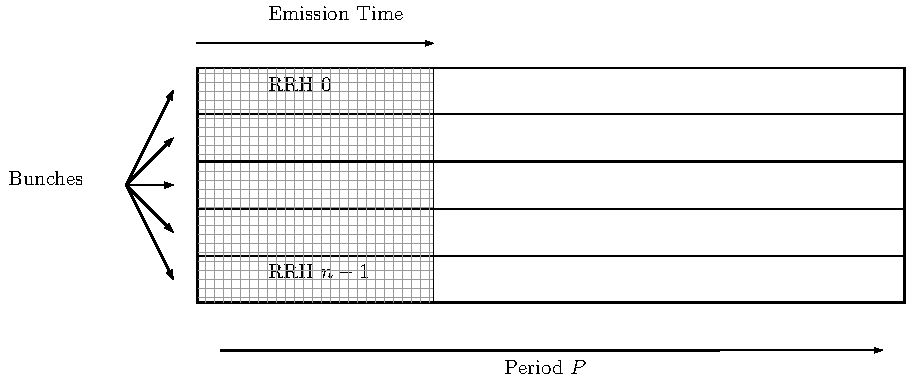
\includegraphics[scale=0.7]{freqgrouped.pdf}
%     \caption{Grouped assignment of the bunches to the RRH.}   \label{fig:freqG}
%  \end{figure}
%
%
%We kept the same parameters than in the two previous experiments (see~\ref{sec:parameters}) and we made an experiment to show the impact of this algorithm on the BE traffic. Fig~\ref{fig:res1} shows us the distribution of latency for BE PDUs with this algorithm.
%
%      \begin{figure}[h]
%\centering
%      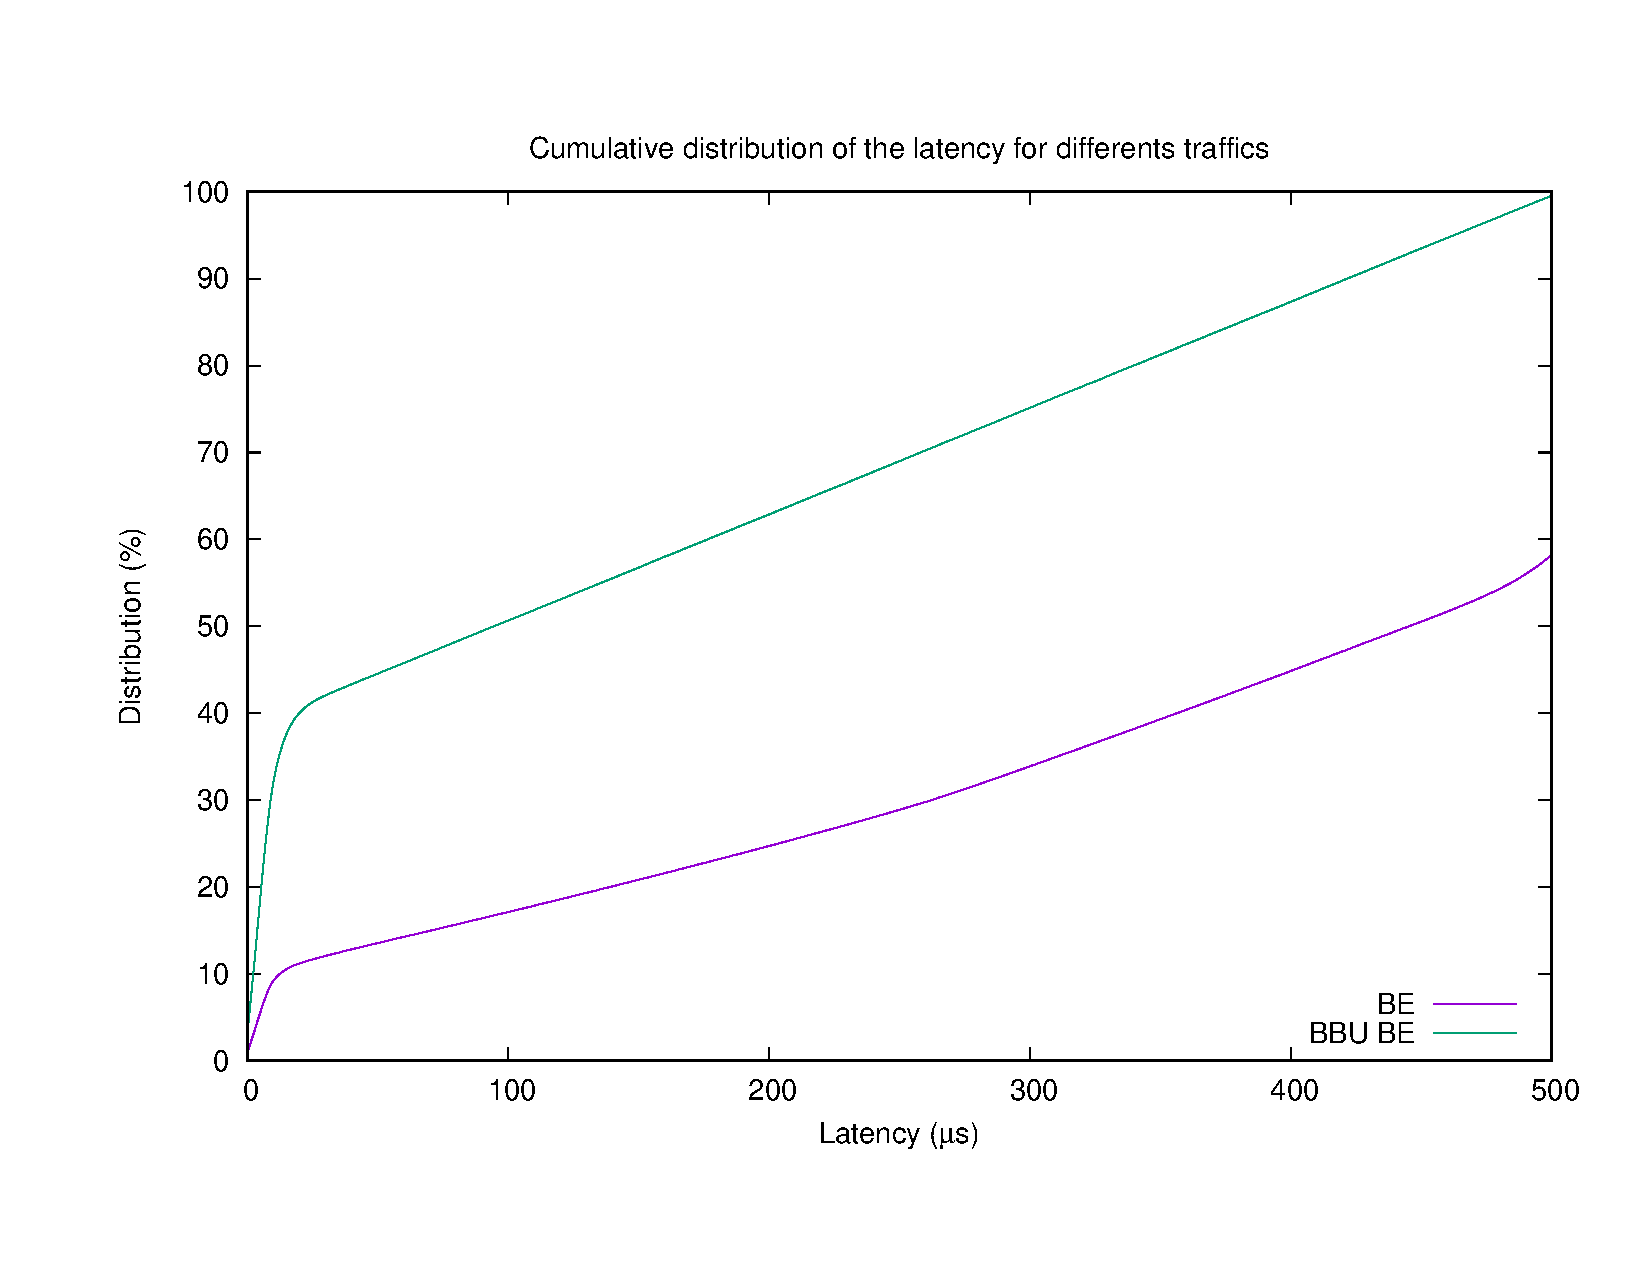
\includegraphics[scale=0.4]{res1.pdf}
%     \caption{Impact of the naive reservation algorithm on the Best effort PDUs.}   \label{fig:res1}
%  \end{figure}
%
%As we can see, the BE traffic is highly penalized by this algorithm, indeed, while almost $100\%$ of the BE PDUs have a latency to less than $200 \mu$s with the full opportunistic method (see fig~\ref{fig:oport}), here, more than half of the BE PDUs are be buffered more than $200\mu s$. Those performances are explained by the structure of the algorithm. The messages are grouped together, and with our parameters, $K = 2\times n$. It creates a long sequence of slots during which there is no free containers in the ring. 
%
%To improve the BE PDUs latnecy, we propose a {\bf splited reservation algorithm} that balances the load of the CRAN traffic over the period. Instead of giving some close BBU-offsets for all routes $i$, with $v$ the datacenter, we now uniformly distribute the different BBU-offsets in the period. Each couple BBU-RRH is still assigned to its bunch, but we split the BBU-offsets of $\frac{P}{n}$. Also, if $2 \times n < K$, the RRH are balanced over the bunches by the same way, we try to give a bunch to a RRH each $\frac{K}{2\times n}$ buches.
%
%   \begin{figure}[!h]
%\centering
%      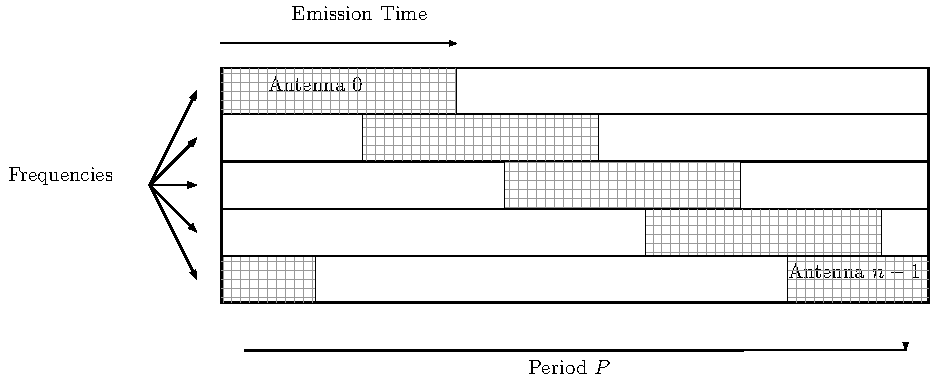
\includegraphics[scale=0.7]{freqsplited.pdf}
%     \caption{Splited assignment of the bunches to the RRH.}   \label{fig:freqS}
%  \end{figure}
%  
%  On fig~\ref{fig:res2} one can observe the performance of this algorithm on the BE PDUs latency. Once again, to have a reference point, we take the same parameters for the simulation. 
%
% \begin{figure}[h]
%\centering
%      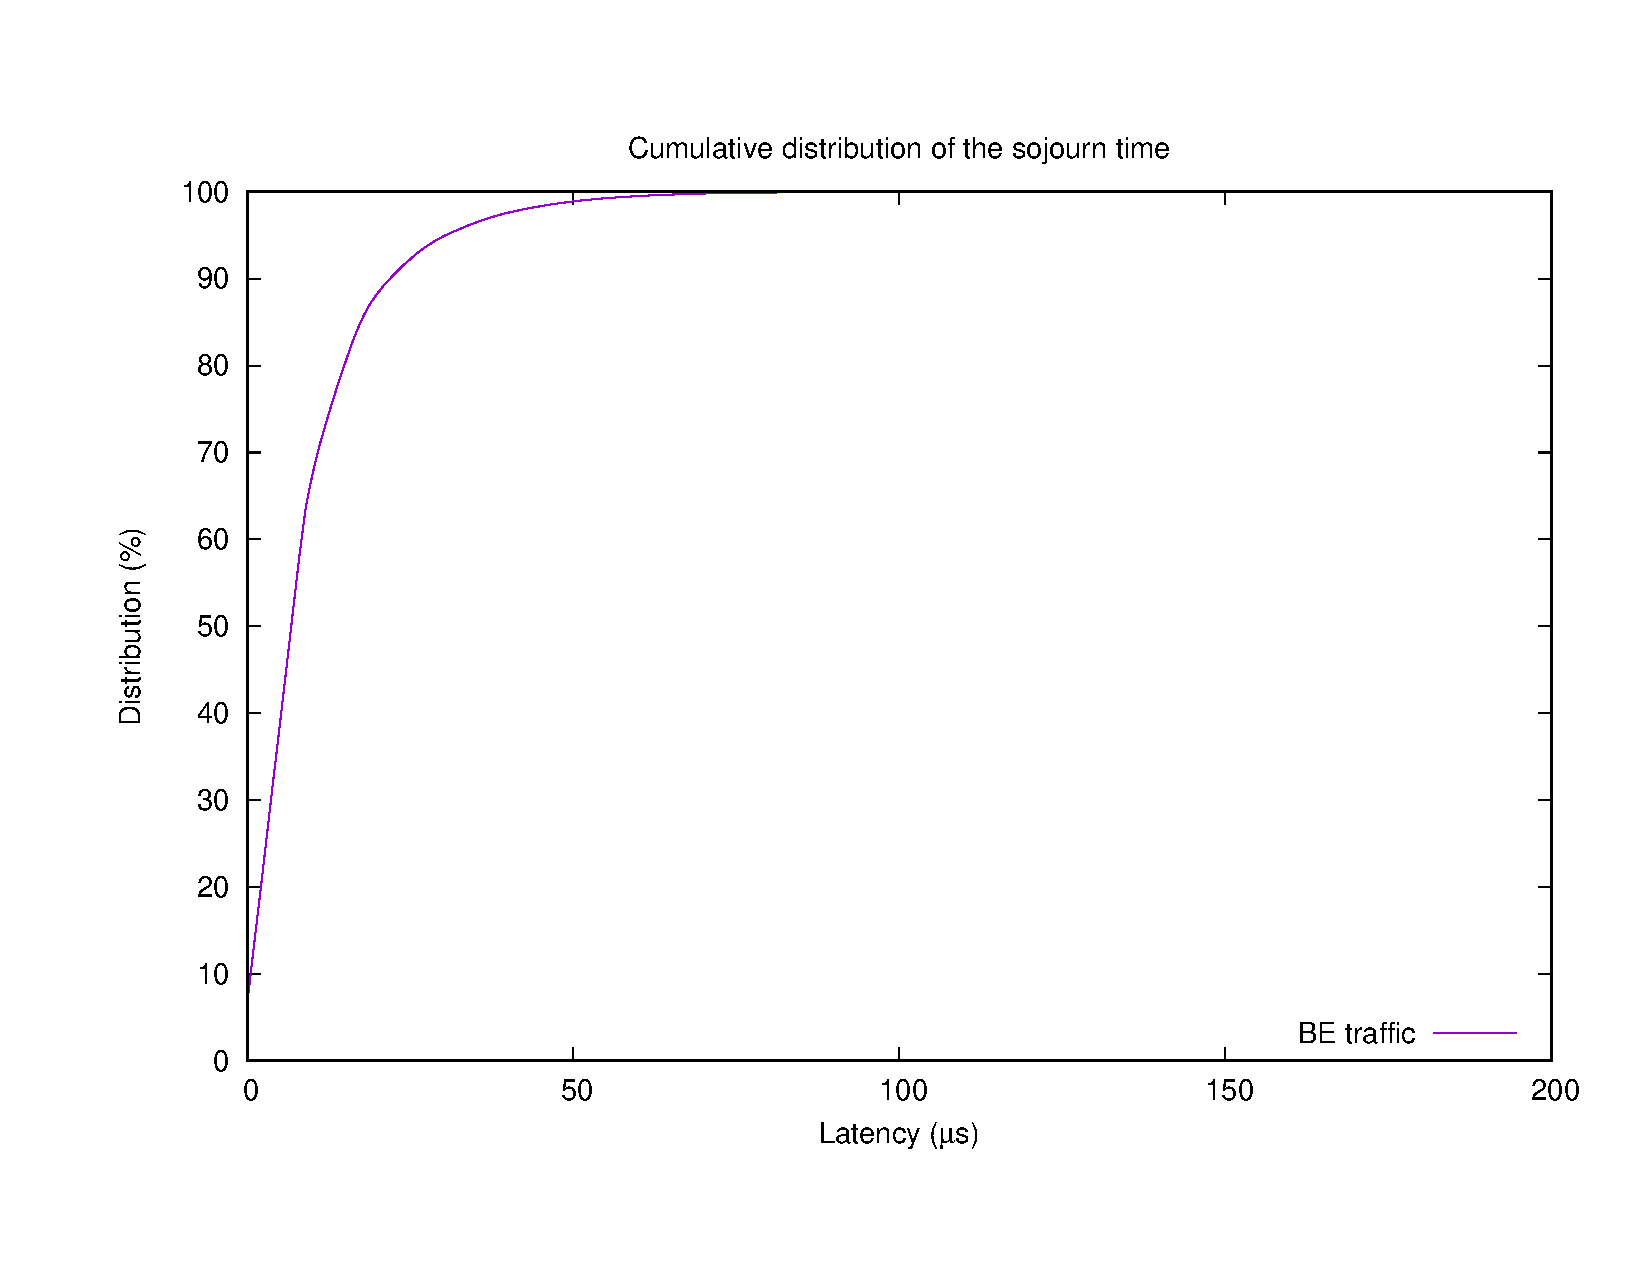
\includegraphics[scale=0.4]{res2.pdf}
%     \caption{Impact of the splited reservation algorithm on the Best effort.}   \label{fig:res2}
%  \end{figure}
%  
%  As we can see, thelatency of the BE PDUs is highly better with this this algorithm. Indeed almost $100\%$ of CRAN PDUs have a latency of less than $50\mu$s which is better than the full opportunistic method. Thus, we decreased the latency of every kind of traffic.
%
%\subsection{With more antennas}
%\label{sec:optialgo}
% In this section, we study the case $n > \frac{K}{2}$, we want to assign more than one RRH to a bunch. 
% Let us consider a particular behavior of the ring. Instinctively, we can think that if we have enough space in the period for many traffics on the same frequency that is, $ET \le \frac{P}{2}$, we can assign several couples BBU-RRH to the same bunch.
%
% Let us take $ET =  \frac{P}{2}$ and $n = \frac{K}{2} + 1$. We assign a bunch to each $\frac{K}{2}$ first RRH and we have only one RRH left. Then, we only look at one bunch, on which we want to add the new couple BBU-RRH. 
% 
% We take a ring with two nodes $A$ and $B$. We simplify the model to only look at the behaviour of one bunch, thus, both of the nodes alternatively emits some containers every slots, during $ET$ slots in the period $P$. We assume that $A$ emits a time $1$ during $ET$ slots. This container arrives in $B$ at $\omega(A,B)$, that is  $[t(B,r_A)]_{P,K} = [\omega(A,B);\omega(A,B)+ET]$. Then, $B$ can immediately emit its containers at time $\omega(A,B)+ET$. This containers from $B$ arrives at $A$ at time $\omega(A,B)+ET + \omega(B,A) = ET + RS$, and thus, $[t(A,r_B)]_{P,K} = [ET + RS;ET + RS + ET] = [ET+RS; RS + P] = [ET + RS; RS] \mod P$. Since $[t(A,r_A)]_{P,K} = [1;ET]$, there is a collision at the interval $[1;RS]$ in the period between the two traffics from $A$ and $B$.
%  \begin{figure}[h]
%\centering
%      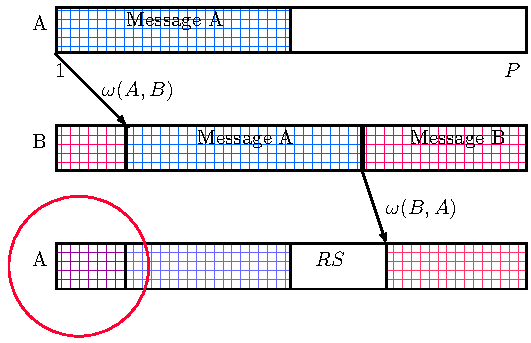
\includegraphics[scale=0.7]{rs.pdf}
%     \caption{Collision between two routes on the same bunch when the period is too small.}   \label{fig:proofrs}
%  \end{figure}
%
% 
% 
% As we have just noted, if several RRH share the same bunch, the period must have an additional budget in addition to the time needed to send the messages. Let us study the size of the additional budget.
% \begin{prop}
% If several RRH shares a bunch, it is possible set the offsets of the routes such that there is no collisions between the messages if $P \ge n\times ET + RS$ , with $n$ the number of RRHs.
% \end{prop}
% \begin{proof}
% We seek to show that proposition by induction.
% 
% {\bf Base case:} For $n = 2$, the proof of the previous example shows us that it is possible to assign two RRH on the same bunch with $P = 2\times ET + RS$.
% 
% {\bf Induction step:}  We consider that we have a bunch shared by $n$ RRH, with a period of size $P= n\times ET + RS$. We want to show that if we want to add one RRH to the bunch, we need a period of size at least $P = (n+1)\times ET + RS$. If we look at the sequence period of the bunch with $n$ RRH. We can observe that this sequence is the same in every nodes, shifted of the length of the routes between two nodes. For instance, if we take two nodes $A$ and $B$, the sequence in $A$ is the same that the sequence in $B$ shifted of $\omega(A,B)$.
% 
%   \begin{figure}[h]
%\centering
%      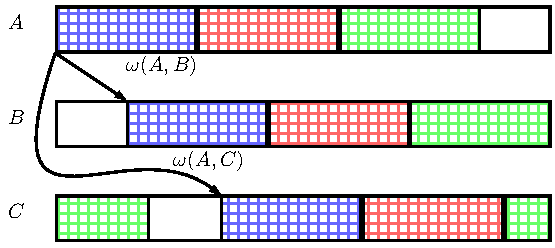
\includegraphics[scale=0.7]{period1.pdf}
%     \caption{An example of sequence with n = 3.}   \label{fig:proofperiod1}
%  \end{figure}
%   
% Thus, if we add $ET$ slots in this bunch, the periodic emissions of all others nodes are not impacted, there is just a new interval in the sequence.
% 
%   \begin{figure}[h]
%\centering
%      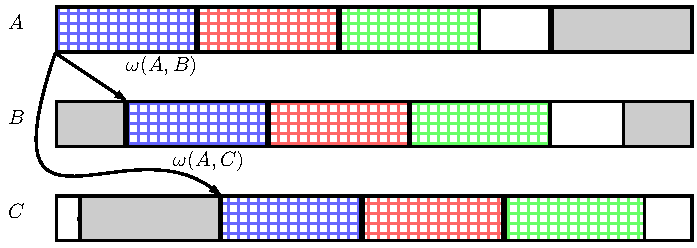
\includegraphics[scale=0.7]{period2.pdf}
%     \caption{The same sequence with n = 4.}   \label{fig:proofperiod2}
%  \end{figure}
%  Note that a station can send some traffic from more than one RRH, the figures ~\ref{fig:proofperiod1} and \~ref{fig:proofperiod2} are just an example, but this proof stays the same.
% \end{proof}
% 
%Considering those results, we propose an algorithm to allow several RRH to share the same bunch, as long as $P \ge n\times ET + RS$. 
%Since we need $RS$ slots on a each bunch with at least an RRH to assign another RRH to this latter, it is interesting to fill as far as possible the bunches. We then compute the number of bunches needed to carry the number of RRH $n$. Then, the algorithms tries to balance those bunches into the macro-slot, i.e. it avoids to group the used bunches together.
%The used bunches have $RS$ or more free slots in the period. Thus, the algorithm subsequently balance BBU-offsets of the first RRH of each bunch, with the same idea than the splited algorithm. We call this algorithm the {\bf full repartition algorithm}. 
%
%   \begin{figure}[h]
%\centering
%      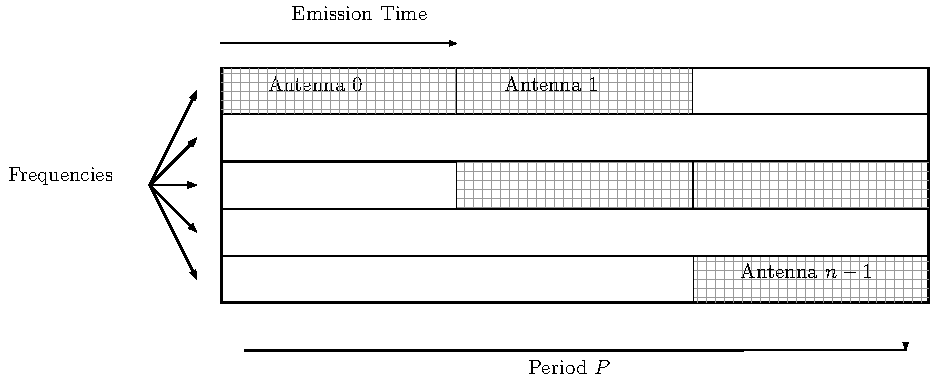
\includegraphics[scale=0.7]{optimalgo.pdf}
%     \caption{Organization of the bunches with the balancing algorithm.}   \label{fig:optimalgo}
%  \end{figure}
%  
%  We want to observe the impact of this algorithm on BE traffic. Since our previous parameters did not allow several RRH to share a bunch, we now set $ET = 200$, that correspond to a C-RAN flow of $2$Gbps. This is not out of context since the exact split (the C-RAN split is the degree of centralization of the computation units in the cloud) of the C-RAN is not fully determined yet~\cite{REF}.\todo {la ref} To keep a load similar to the load in the previous experiment, we set the number of RRH to $n=12$. The others parameters are all the one described in the sec~\ref{sec:parameters}.
%  The following experiment shows us the impact of the balancing algorithm on the BE traffics. We chose to compare those results to a simulation with the same parameters but with the full opportunistic method of sec~\ref{sec:fullopport}.
%  
%   \begin{figure}[h]
%\centering
%      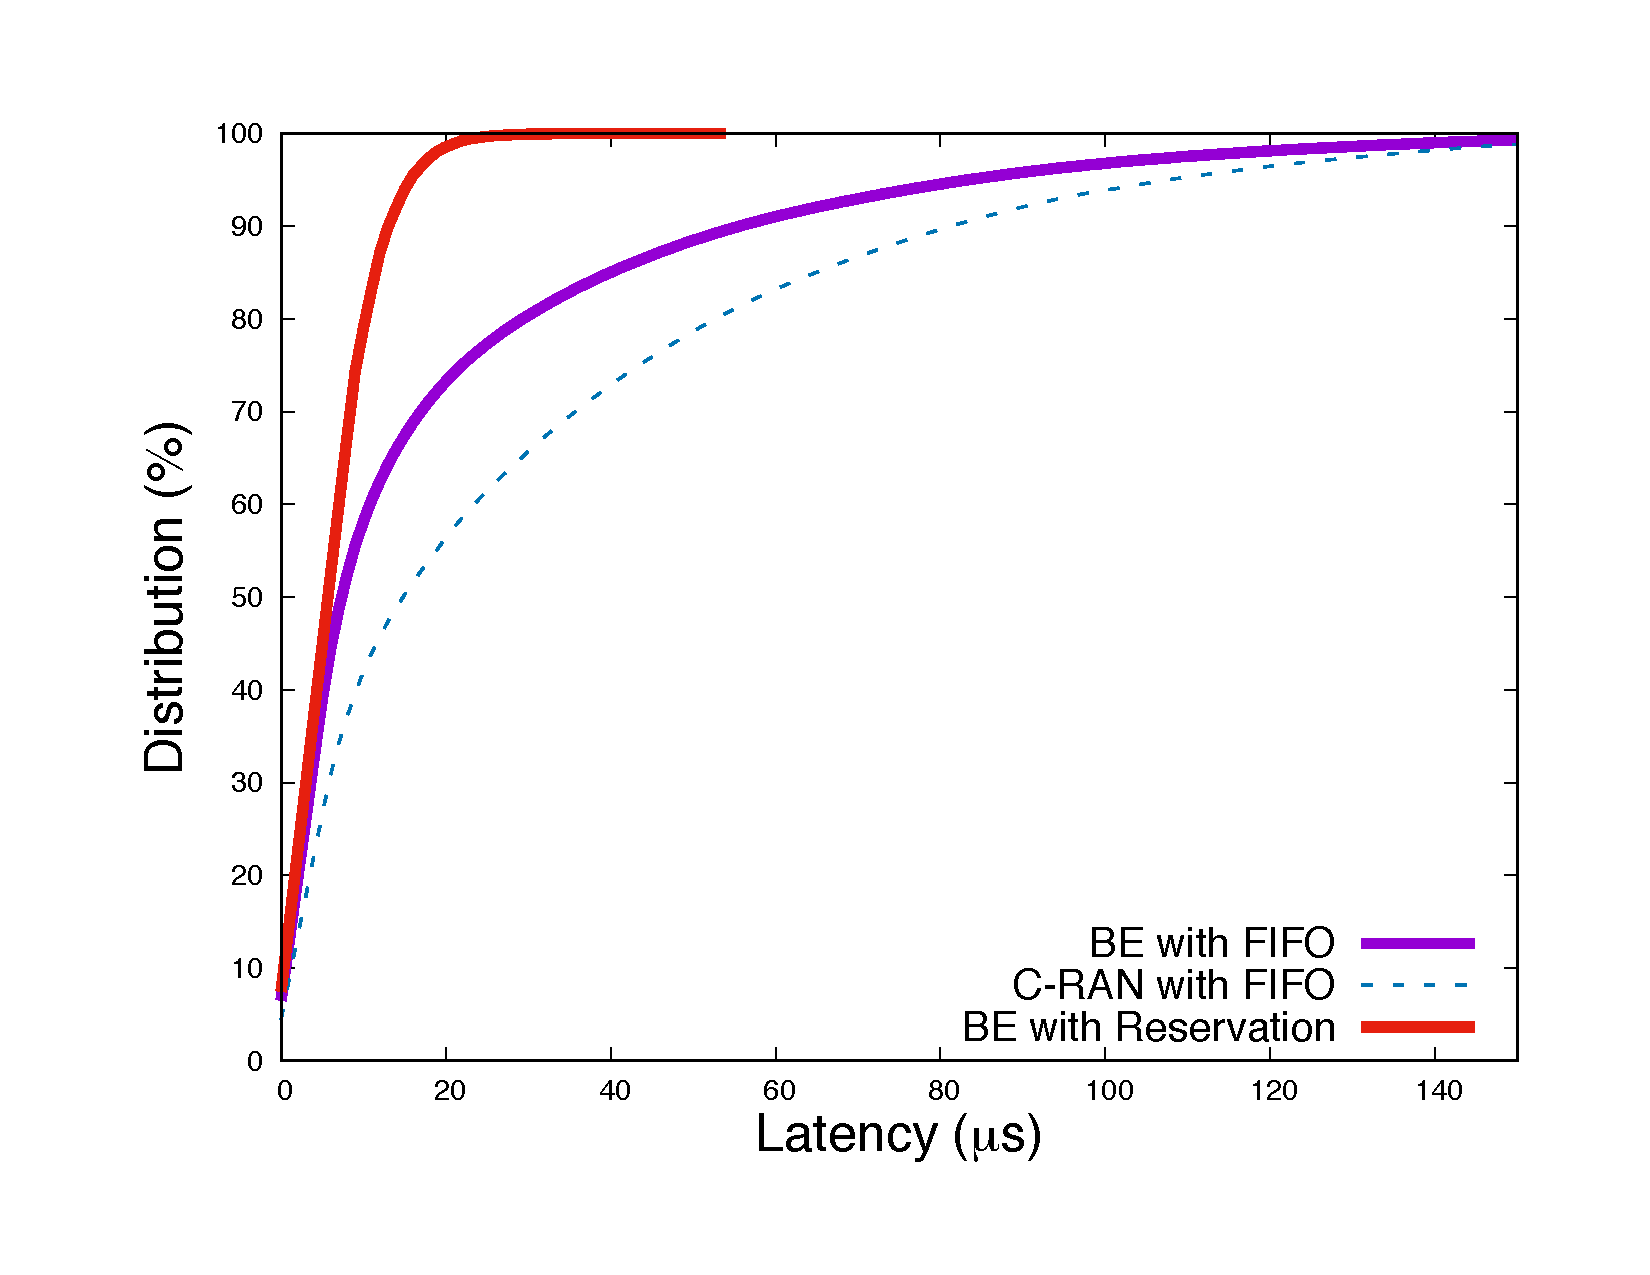
\includegraphics[scale=0.4]{optim.pdf}
%     \caption{Balancing algorithm performance on the N-GREEN optical ring.}   \label{fig:optimres}
%  \end{figure}
%  
%  As fig~\ref{fig:optimres} shows, the full repartition algorithm ensures a lower latencye to BE PDUs than the full opportunistic method, which gave the best result for the BE traffic. Indeed, since we remove the random aspect of the C-RAN PDUs generation, we balanced the load over the period an then increased the BE performances while we totally removed the C-RAN PDUs latency.
  
  \bibliographystyle{ieeetr}
\bibliography{src}

\end{document}